\begin{figure}[tb]
    \centering
    \begin{subfigure}[tb]{0.48\textwidth}
        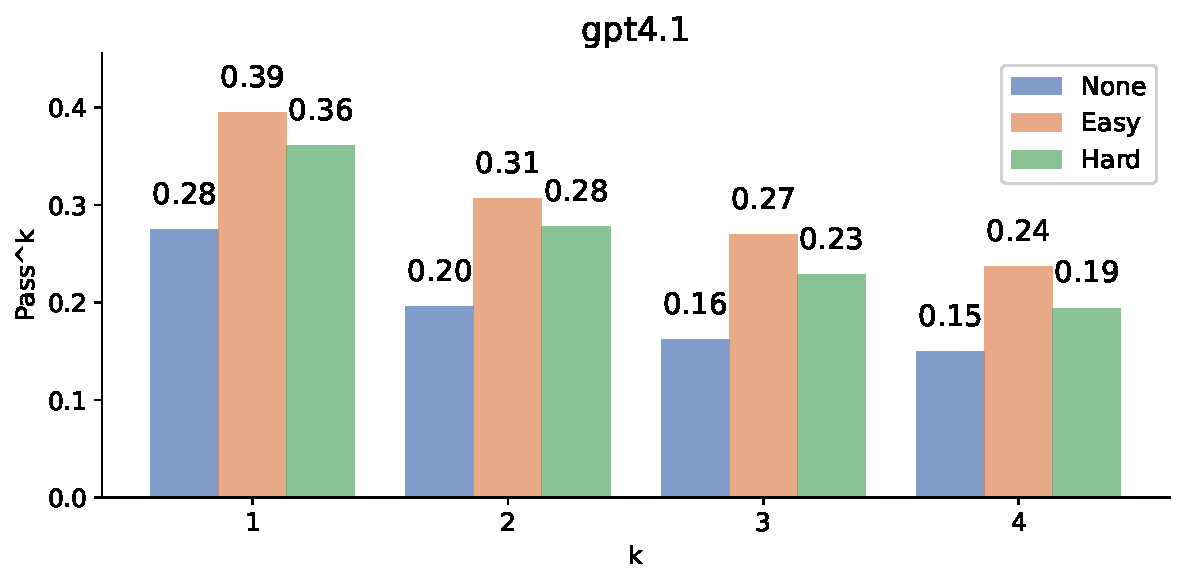
\includegraphics[width=\textwidth]{figures/results/pass_k_vs_k_per_persona_telecom_gpt-4.1-2025-04-14.pdf}
    \end{subfigure}
    \hfill
    \begin{subfigure}[tb]{0.48\textwidth}
        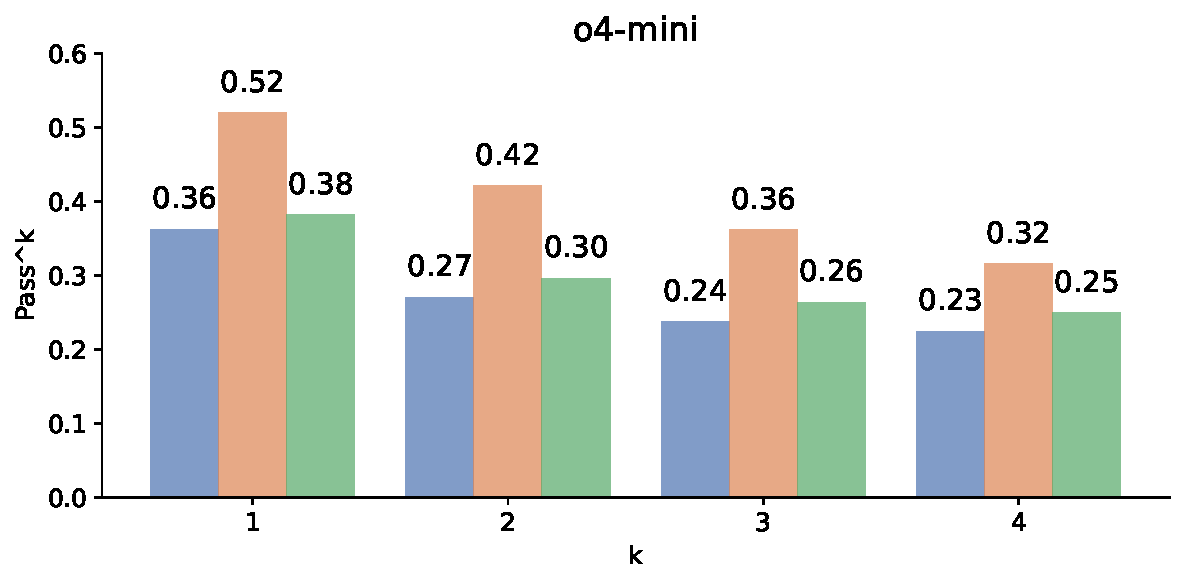
\includegraphics[width=\textwidth]{figures/results/pass_k_vs_k_per_persona_telecom_o4-mini-2025-04-16.pdf}
    \end{subfigure}
    \vspace{0.5em}
    \begin{subfigure}[tb]{0.48\textwidth}
        \centering
        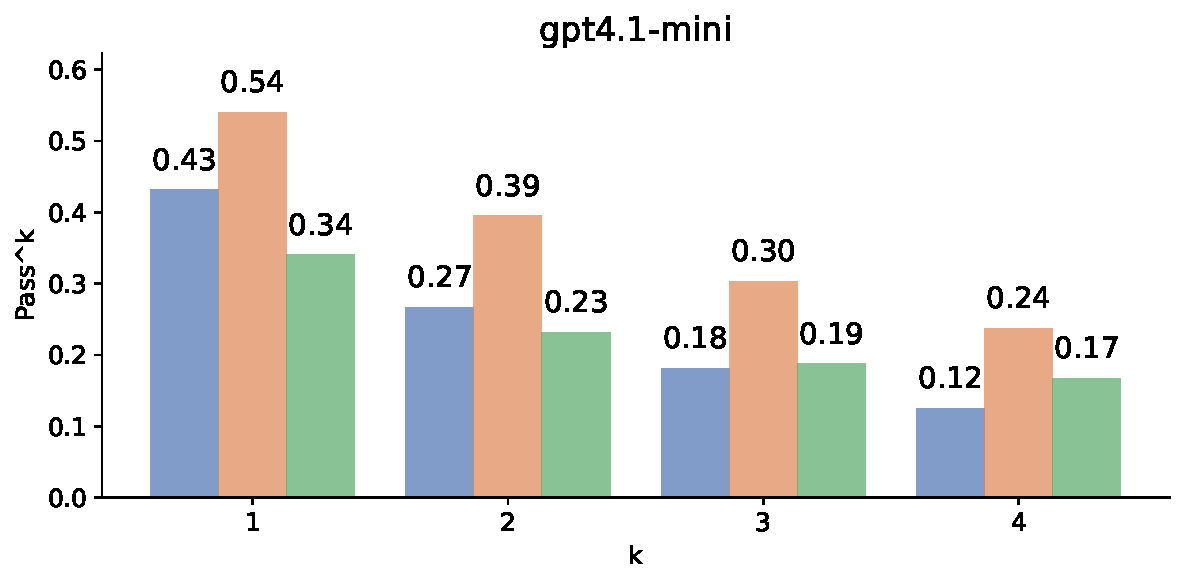
\includegraphics[width=\textwidth]{figures/results/pass_k_vs_k_per_persona_telecom_gpt-4.1-mini-2025-04-14.pdf}
    \end{subfigure}
    \hfill
    \begin{subfigure}[tb]{0.48\textwidth}
        \centering
        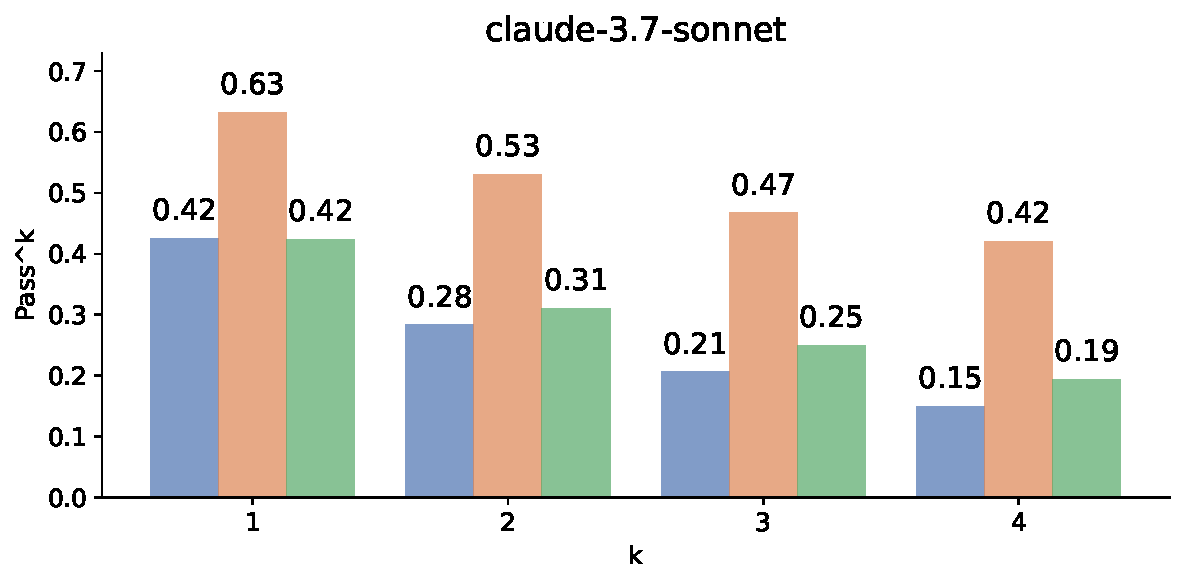
\includegraphics[width=\textwidth]{figures/results/pass_k_vs_k_per_persona_telecom_claude-3-7-sonnet-20250219.pdf}
    \end{subfigure}
    \vspace{-0.8em}
    \caption{\gptmodelshort (top left), \ofourmodelshort (top right), \gptminishort (bottom left), and \claudesonnetshort (bottom right) \passk per persona type for the \telecom domain. Performance is shown across different persona types, highlighting how different user characteristics affect success rates.}
    \label{fig:telecom_persona_results}
    \vspace{-1em}
\end{figure} 
